\documentclass[english, DIV=13]{scrreprt}

\usepackage[utf8x]{inputenc}
\usepackage[T1]{fontenc}
\usepackage{lmodern}
\usepackage{microtype}
\usepackage{xspace}
\usepackage[binary-units=true]{siunitx}
\usepackage{graphicx}
\usepackage{hyperref}
\usepackage{todonotes}
\usepackage{epstopdf}
\usepackage{array}
\usepackage{multicol}
\usepackage{multirow}
\usepackage{tabularx} % tabular with automatic line-break
\newcolumntype{Y}{>{\centering\arraybackslash}X} % centered column
\usepackage{amsmath}
\usepackage{grffile} % better name handling with graphicx
\usepackage{currfile} % provides relative file inclusion for tikzscale
\usepackage{listings}
\lstset{%
    basicstyle=\scriptsize\ttffamily,
    breaklines=true
}

\usepackage{tikz}
\usepackage{pgfplots}
\usepackage{pgfplots}
\usepackage{tikzscale}
\pgfplotsset{compat=newest}
\usetikzlibrary{plotmarks}
\usepackage{rotating}
\usepackage[absolute,overlay]{textpos}
\usepackage{circuitikz}

% Math symbols
\usepackage{amsmath}
\usepackage{amssymb}
\usepackage{amsthm}
\DeclareMathOperator*{\argmin}{arg\,min}
\DeclareMathOperator*{\argmax}{arg\,max}
\newcommand\norm[1]{\left\lVert#1\right\rVert}

% Sets
\newcommand{\Z}{\mathbb{Z}}
\newcommand{\R}{\mathbb{R}}
\newcommand{\Rn}{\R^n}
\newcommand{\Rnn}{\R^{n \times n}}
\newcommand{\C}{\mathbb{C}}
\newcommand{\K}{\mathbb{K}}
\newcommand{\Kn}{\K^n}
\newcommand{\Knn}{\K^{n \times n}}

% Unit vectors
\usepackage{esint}
\usepackage{esvect}
\newcommand{\kmath}{k}
\newcommand{\xunit}{\hat{\imath}}
\newcommand{\yunit}{\hat{\jmath}}
\newcommand{\zunit}{\hat{\kmath}}
\newcommand{\uunit}{\hat{\umath}}

% rot & div & grad & lap
\DeclareMathOperator{\newdiv}{div}
\newcommand{\divn}[1]{\nabla \cdot #1}
\newcommand{\rotn}[1]{\nabla \times #1}
\newcommand{\grad}[1]{\nabla #1}
\newcommand{\gradn}[1]{\nabla #1}
\newcommand{\lap}[1]{\nabla^2 #1}

% Elec
\newcommand{\B}{\vec B}
\newcommand{\E}{\vec E}
\newcommand{\EMF}{\mathcal{E}}
\newcommand{\perm}{\varepsilon} % permittivity

\newcommand{\bigoh}{\mathcal{O}}
\newcommand\eqdef{\triangleq}

\DeclareMathOperator{\newdiff}{d} % use \dif instead
\newcommand{\dif}{\newdiff\!}
\newcommand{\fpart}[2]{\frac{\partial #1}{\partial #2}}
\newcommand{\ffpart}[2]{\frac{\partial^2 #1}{\partial #2^2}}
\newcommand{\fdpart}[3]{\frac{\partial^2 #1}{\partial #2\partial #3}}
\newcommand{\fdif}[2]{\frac{\dif #1}{\dif #2}}
\newcommand{\ffdif}[2]{\frac{\dif^2 #1}{\dif #2^2}}
\newcommand{\constant}{\ensuremath{\mathrm{cst}}}


\title{LELEC2103}
\subtitle{Project in Electricity 3 : Electronic systems}
\author{Gaëtan Cassiers\and Antoine Paris}
\date{\today}

\begin{document}
\maketitle

\chapter{Introduction}

\chapter{Gameplay and features}
Our game is inspired by an existing game available on most smartphones and tablets
and developped by Ketchapp. Figure~\ref{fig:original-game} is a screenshot from this game.
In this original version of the game, the player (represented by the yellow cube on figure
~\ref{fig:original-game}) has to place itself correctly on the white structure in order
to fit in the hole of the wall coming in his direction at a constant speed. The objective
is to pass in as much wall as possible. Passing a wall gives 1 point, failing to pass a
wall makes the score starting back at 0.

Our version of the game differs from the original one in several aspects. First, this
is a two-players collaborative game. Second, a game only lasts a finite amount of time
and the two players can control the speed of the wall using the accelerometer.
Finally, failing to pass a wall only decreases the current score by 1.

\begin{figure}
    \centering
    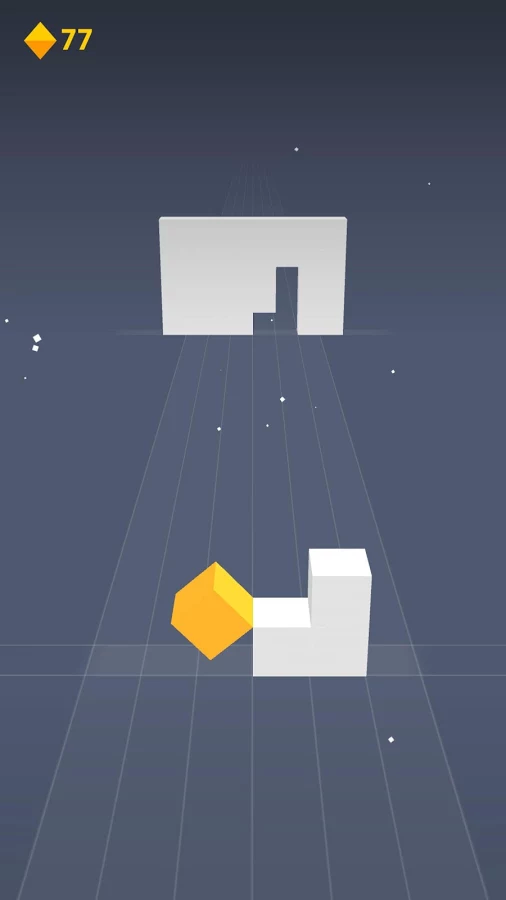
\includegraphics[width=0.4\textwidth]{img/original-game}
    \caption{Screenshot of the orginal game by Ketchapp.}
    \label{fig:original-game}
\end{figure}

\chapter{Network interface}
The way the two players communicate with each other is illustrated in figure~\ref{fig:
comm-scheme}. The approach taken here is client-server based. The server is responsible
for all the logic of the game and maintains an object representing the state of the game.
Centralizing computations in this way ensures a complete synchronization between clients.

A complete communication protocol was rigorously defined by the two groups. This
protocol defines an handshake procedure between a client and the server to ensure both
sides are ready before starting. Once the game has started, the two clients can send
messages to the server based on user inputs (accelerometer values, touch, or gesture).
The server then performs some computations on the game state such as computing player
positions, speed of the wall, remaining time, score, etc. Finally, the server
broadcasts the parts of the game state which changed.

On the practical side, one Raspberry-Pi runs both the server and a client while the other
one only runs a client.

\begin{figure}
    \centering
    \includegraphics[width=1.0\textwidth]{img/global_comm_scheme_cropped.pdf}
    \caption{Block diagram of the network communication.}
    \label{fig:comm-scheme}
\end{figure}

\chapter{Global view of the client system}
The global view of the client system is represented in figure~\ref{fig:global-desktop}
and figure~\ref{fig:global-device}. Through the network interface described in the
previous section, the client builds its own image of the game state. This client game
state is then fed to the rendering subsystem which produces a 3D image. This image
is then compressed and sent to the hardware interface.

One of the strength of our system is this hardware interface. This abstraction offers
a common layer to communicate both with a PC or a device. This eased a lot the development
process.

\begin{figure}
    \centering
    \includegraphics[width=0.6\textwidth]{img/block_global_desktop_cropped.pdf}
    \caption{Block diagram of the client, when running on a PC.}
    \label{fig:global-desktop}
\end{figure}

\begin{figure}
    \centering
    \includegraphics[width=0.6\textwidth]{img/block_global_device_cropped.pdf}
    \caption{Block diagram of the client, when running the raspberry-pi/DE0-Nano system.}
    \label{fig:global-device}
\end{figure}

\chapter{Rendering subsystem}

\begin{figure}
    \centering
    \includegraphics[width=0.6\textwidth]{img/block_rendering_cropped.pdf}
    \caption{Pipeline for the rendering of the video.}
\end{figure}

\chapter{Compression subsystem}

\begin{figure}
    \centering
    \includegraphics[width=0.8\textwidth]{img/compression_scheme_cropped.pdf}
    \caption{Principle view of the compression scheme.}
\end{figure}

\chapter{SPI slave subsystem}

\begin{figure}
    \centering
    \includegraphics[width=0.5\textwidth]{img/spi_state_machine_cropped.pdf}
    \caption{State machine for the SPI communication protocol.}
\end{figure}

\chapter{Display management}

\begin{figure}
    \centering
    \includegraphics[width=\textwidth]{img/display_manager_cropped.pdf}
    \caption{Block diagram of the display management and synchronization system.}
\end{figure}

\chapter{Input detection subsystem}

\begin{figure}
    \centering
    \includegraphics[width=0.5\textwidth]{img/tasks_mC_cropped.pdf}
    \caption{Tasks and their relationships on the uC/OS-II operating system.}
\end{figure}

\chapter{Player pictures acquisition}

\begin{figure}
    \centering
    \includegraphics[width=0.5\textwidth]{img/block_pictures_cropped.pdf}
    \caption{Block diagram of the picture acquisition subsystem.}
\end{figure}

\chapter{Conclusion}

\end{document}
